\section{可去奇点定理}
\stfhIndex{I236}{ke^qu^qi^dian^ding^li}{可去奇点定理（removal singularity theorem）}
\label{sec:removable-singularity-theorem}

本节证明可去奇点定理。仍令 $D$ 表示开单位圆盘或满足
$\partial D=(-1,1)$ 的开半圆盘。设 $(M,\omega,J)$ 为\emph{不必紧}的殆凯勒
流形，$L\subset M$ 为无边界紧拉格朗日子流形。假设 $(M,\omega)$ 驯服，因而带有相容的 $J$，使
$g=\omega(\cdot,J\cdot)$ 所定义的 $(M,J,g)$ 在定义 8.7.7 的意义下驯服。
\begin{theorem}\label{thm:ch8-removable-singularity-w1p}
若 $u:D\setminus\{0\}\to M$ 为 $J$-全纯映射，$u(\partial D)\subset L$，像包含于紧集 $K$，且 $\int_{D\setminus\{0\}}|du|^2<\infty$，则 $u\in W^{1,p}$ 对某个 $p>2$ 成立。
\end{theorem}
\begin{corollary}\label{cor:ch8-removable-singularity-smooth}
上述 $u$ 光滑延拓到 $D$。
\end{corollary}
\begin{proof}
由定理 8.5.5，只须验证延拓后的 $W^{1,p}$ 映射在 $D$ 上弱 $J$-全纯。由于
$u$ 在 $D^2\setminus\{0\}$ 上光滑且 $J$-全纯，显然
$\int_D|\bar\partial_Ju|^2=0$。为验证边界条件
\eqref{eq:ch8-weak-neumann-condition}，令 $X$ 是 $D$ 上任意光滑向量场，它在
$\mathring D$ 中紧支并且在边界上关于 $g_0$ 垂直于 $R$。因
$u\in W^{1,p}$ 且 $X\in W^{1,2}$，
\[
 \int_D\langle Jdu,\nabla X\rangle
 =\lim_{r\to0}\int_{D\setminus D(r)}\langle Jdu,\nabla X\rangle.
\]
取上半平面的标准坐标 $(x,y)$ 并设 $\partial D\subset\partial\mathbb H$。在
$D\setminus D(r)$ 上用 $\bar\partial_Ju=0$ 并分部积分，得到
\begin{align*}
 \int_{D\setminus D(r)}\langle Jdu,\nabla X\rangle
 &=\int_{D\setminus D(r)}
 \left(\left\langle u_y,\frac{DX}{\partial x}\right\rangle
 -\left\langle u_x,\frac{DX}{\partial y}\right\rangle\right)\,dx\,dy\\
 &=\int_{\partial(D\setminus D(r))}
 \left(-\langle u_x,X\rangle dx+\langle u_y,X\rangle dy\right)\\
 &\quad+\int_{D\setminus D(r)}
 \left(\left\langle\frac D{\partial x}u_y,X\right\rangle
 -\left\langle\frac D{\partial y}u_x,X\right\rangle\right)\,dx\,dy\\
 &=-\int_{\partial(D\setminus D(r))}\langle u_x,X\rangle dx
 +\langle u_y,X\rangle dy\\
 &=\int_{\partial D(r)}\langle u_x,X\rangle dx-\langle u_y,X\rangle dy.
\end{align*}
倒数第二步用推论 7.3.3 的
$D_xu_y=D_yu_x$；最后一步用 $X\perp_{g_0}R$ 以及 $u_x\in TR$，故
$\langle u_x,X\rangle=0$。最后
\[
 \left|\int_{\partial D(r)}\langle u_x,X\rangle dx-\langle u_y,X\rangle dy\right|
 \leq2\|X\|_{C^0}L(u|_{\partial D(r)}),
\]
下述库朗--勒贝格引理给出使右端趋零的子列，证明完毕。
\end{proof}

为证明定理 8.6.1，先给出下面这个有用引理；其中半圆盘版本取自 (Oh92)。
\begin{lemma}[库朗--勒贝格]\label{lem:ch8-courant-lebesgue}\leavevmode\par
\stfhIndex{I088}{ku^lang^lei^bei^ge^yin^li}{库朗--勒贝格引理（Courant–Lebesgue lemma）}
给定 $0<\sigma<1$。若 $u\in W^{1,2}(D,M)$，或
$u\in W^{1,2}((D,\partial D),(M,L))$，且
$\int_{D(\sigma)}|du|^2\leq\Gamma$，则存在 $\rho\in[\sigma^2,\sigma]$ 使
$L(u|_{|x|=\rho})^2\leq C\Gamma/\log(1/\rho)$，其中 $C=C(\Gamma)$，并记
$L(\gamma)(s)=\int|\gamma'|dt$。
\end{lemma}
对 $W^{1,2}$ 映射，$L(u|_{|x|=\rho})^2$ 关于 $\rho$ 几乎处处有定义，但未必处处有定义。把引理应用于
$\cdots\leq\sigma^n<\sigma^{n-1}<\cdots<\sigma<1$，特别可得到一列
$\rho_i$，使圆周曲线 $u|_{|x|=\rho_i}$ 的长度趋于零。
\begin{proof}
只论半圆盘。以极坐标并用赫尔德不等式，
\begin{align*}
 \int_{\sigma^2}^{\sigma}\frac{L(u|_{|x|=r})^2}{r}\,dr
 &=\int_{\sigma^2}^{\sigma}\frac1r
 \left(\int_0^\pi\left|u_\theta\right|_{|x|=r}d\theta\right)^2dr\\
 &\leq\int_{\sigma^2}^{\sigma}\frac1r
 \left(\int_0^\pi|u_\theta|^2_{|x|=r}d\theta\cdot\pi\right)dr\\
 &=\pi\int_{\sigma^2}^{\sigma}\int_0^\pi
 \left|\frac1r u_\theta\right|^2_{|x|=r}r\,dr\,d\theta
 \leq\pi\int_{D(\sigma)\setminus D(\sigma^2)}|du|^2\leq\pi\Gamma.
\end{align*}
因此长度平方在 $[\sigma^2,\sigma]$ 上几乎处处有定义。若它几乎处处大于
$C\Gamma/\log(1/r)$，则
\[
 \int_{\sigma^2}^{\sigma}\frac{L(u|_{|x|=r})^2}{r}dr
 >\int_{\sigma^2}^{\sigma}\frac{C\Gamma}{r\log(1/r)}dr=C\Gamma\log2.
\]
取 $C\log2>\pi$ 即矛盾。
\end{proof}

\begin{proof}[定理 8.6.1 的证明]
由法图引理，
\[
 \lim_{r\to0}\int_{D\setminus D(r)}|du|^2
 \longrightarrow\int_{D\setminus\{0\}}|du|^2<\infty.
\]
因此可取充分小的 $r_0>0$，使
$\int_{D(r_0)\setminus\{0\}}|du|^2<\epsilon$，其中 $\epsilon$ 是
$\epsilon$-正则性定理中的常数。
\begin{lemma}\label{lem:ch8-image-enters-darboux-neighborhood}
给定 $L$ 的达布邻域 $U$，充分小的 $r_1<r_0$ 满足
$\operatorname{Im}(u(D(r_1)\setminus\{0\}))\subset U$。
\end{lemma}
\begin{proof}
反设有 $|z_i|=:r_i\to0$ 而 $u(z_i)\notin U$。因\emph{$K\cap L$ 紧}，存在
$\delta>0$ 使 $\operatorname{dist}(L\cap K,M\setminus U)\geq\delta$，故
$\operatorname{dist}(u(z_i),L)\geq\delta$。这个 $\delta$ 与具体 $u$ 无关，只依赖于
$U\cap K,J,\omega,L$。库朗--勒贝格引理给出 $s_i<r_i<s_i'$，且
$L(u|_{|z|=s_i}),L(u|_{|z|=s_i'})<\delta/4$。由边界条件，
\[
 \max_{|z|=s_i,s_i'}\operatorname{dist}(u(z),L)\leq\delta/4.
\]
于是 $\operatorname{Im}u\cap B(u(z_i),\delta/2)$ 是球中以 $u(z_i)$ 为中心的恰当
$J$-全纯曲线。下一节命题 8.7.10 给出
\[
 \operatorname{Area}\bigl(\operatorname{Im}u\cap B(u(z_i),\delta/2)\bigr)
 \geq C(\delta/2)^2.
\]
若取 $0<\epsilon<C(\delta/2)^2$，这与左端不超过
$\operatorname{Area}(u)\leq\epsilon$ 矛盾。
\end{proof}
把 $D(r_1)$ 共形放大为 $D$，并相应重参数化 $u$，可假设
$\int_{D\setminus\{0\}}|du|^2<\epsilon$。在 $U$ 上取
$\omega=-d\beta$ 且 $\beta|_L=0$；例如可取余切丛刘维尔 $1$-形式的限制。
令 $A_m=\{z\in D\mid0<r_m\leq|z|\leq1\}$。由于 $u$ 是 $J$-全纯的，我们导出
\begin{equation}
 \begin{split}
 \frac12\int_{A_m}|du|^2
 &=\int_{A_m}u^*\omega\\
 &=-\int_{A_m}u^*d\beta\\
 &=-\int_{S(1)}u^*\beta+\int_{S(r_m)}u^*\beta
   \pm\int_{A_m\cap\{\operatorname{Im}z=0\}}u^*\beta\\
 &=-\int_{S(1)}u^*\beta+\int_{S(r_m)}u^*\beta+0.
 \end{split}
 \label{eq:ch8-semiannulus-stokes}
\end{equation}
\begin{figure}[htbp]\centering
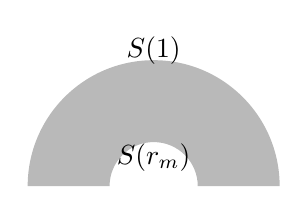
\begin{tikzpicture}[scale=.8]\fill[gray!55] (-2,0) arc[start angle=180,end angle=0,radius=2] -- (.7,0) arc[start angle=0,end angle=180,radius=.7] -- cycle;\node at (0,2.15){$S(1)$};\node at (0,.45){$S(r_m)$};\end{tikzpicture}
\caption{半环域。}\label{fig:ch8-semiannulus}
\end{figure}
最后一项因 $\beta|_L=0$ 消失；这正是拉格朗日条件相较一般全实边界的优势，一般情形需 (Ye94) 的更精细估计。由法图引理，
\[
 \lim_{m\to\infty}\frac12\int_{A_m}|du|^2
 =\frac12\int_{D\setminus\{0\}}|du|^2.
\]
另一方面，
\[
 \left|\int_{S(r_m)}u^*\beta\right|
 \leq\int_0^{2\pi}\left|\beta\left(
 \left.\frac{\partial u}{\partial\theta}\right|_{|z|=r_m}
 \right)\right|\,d\theta
\]
且
\[
 \int_0^{2\pi}\left|\beta\left(
 \left.\frac{\partial u}{\partial\theta}\right|_{|z|=r_m}
 \right)\right|\,d\theta
 \leq C\|\beta\|_{C^0}\int_0^{2\pi}
 \left|\left.\frac{\partial u}{\partial\theta}\right|_{|z|=r_m}\right|\,d\theta
 =C\|\beta\|_{C^0}L(u|_{|z|=r_m}).
\]
回忆在证明开始处所选的 $r_m$ 满足 $L(u|_{|z|=r_m})\to0$，故
$\frac12\int_{D\setminus\{0\}}|du|^2=-\int_{S(1)}u^*\beta
\leq C\|\beta\|_{C^0}L(u|_{|z|=1})$。常数 $C$ 与具体曲线无关。对
$u_r(z)=u(rz)$，得到
\begin{equation}\frac12\int_{D\setminus\{0\}}|du_r|^2\leq C\|\beta\|_{C^0}L(u_r|_{|z|=1}),\label{eq:ch8-rescaled-isoperimetric}\end{equation}
这里 $u_r:D\setminus\{0\}\to M$ 是把 $u|_{0<|z|<r}$ 共形重参数化到单位圆盘所得的
$u_r(z)=u(rz)$。能量的共形不变性给出
\[
 \frac12\int_{D(r)\setminus\{0\}}|du|^2
 =\frac12\int_{D\setminus\{0\}}|du_r|^2,
\]
而长度变换为
\begin{equation}
 \begin{split}
 L(u_r|_{|z|=1})
 &=\int_0^\pi\left|\left.\frac{\partial u_r}{\partial\theta}\right|_{|z|=1}\right|\,d\theta\\
 &=\int_0^\pi r\left|\left.\frac{\partial u}{\partial\theta}\right|_{|z|=r}\right|\,d\theta
 =rL(u|_{|z|=r}).
 \end{split}
 \label{eq:ch8-length-rescaling}
\end{equation}
现在记
\[
 E(r)=\frac12\int_{D(r)\setminus\{0\}}|du|^2,\quad
 L(r)=L(u|_{|z|=r}),\quad A(r)=\operatorname{Area}(u(D(r))).
\]
因 $u$ 为 $J$-全纯，恒有
\begin{equation}E(r)=A(r)=\operatorname{Area}(u|_{0<|z|<r}).\label{eq:ch8-energy-area-identity}\end{equation}
合并前三式得 $A(r)\leq C'rL(r)$，其中 $C'=C\|\beta\|_{C^0}$。因此
$A(r)\leq C'rA'(r)$，等价地 $E(r)\leq C'rE'(r)$，从而
\[
 1\leq C'r\frac1{E(r)}\frac{dE(r)}{dr}.
\]
除以 $C'r$ 并从 $r$ 积分到 $1$，
\[
 \int_r^1\frac1{C's}ds\leq\log E(1)-\log E(r)
 =\log\frac{E(1)}{E(r)};
\]
故若 $\lambda=1/C'$，则 $E(r)\leq E(1)r^\lambda$，即
\begin{equation}\int_{D(|z|\leq r)}|du|^2\leq E(1)r^\lambda,\label{eq:ch8-energy-power-decay}\end{equation}
再由命题 8.4.6 得
\begin{equation}
 |du(z)|^2\leq\frac{C'}{|z|^2}E(1)|z|^\lambda
 =C'E(1)|z|^{\lambda-2}.
 \label{eq:ch8-derivative-power-decay}
\end{equation}
其中 $\lambda>0$，且上式对所有满足 $|z|\leq1/4$ 的 $z$ 成立。于是
\[
 |du(z)|^p\leq C''|z|^{((\lambda-2)/2)p}
 =C''|z|^{p(\lambda/2-1)},
\]
其中 $C''=C'E(1)$。而
\[
 \begin{split}
 \int_0^1\int_0^{2\pi}|z|^{p(\lambda/2-1)}r\,dr\,d\theta
 &=2\pi\int_0^1r^{p(\lambda/2-1)+1}\,dr\\
 &=\frac{2\pi}{p(\lambda/2-1)+2}
 -\lim_{r\to0}2\pi\frac{r^{p(\lambda/2-1)+2}}{p(\lambda/2-1)+2}.
 \end{split}
\]
若能取 $p>2$ 使 $p(\lambda/2-1)+2>0$，则此极限有限。若
$\lambda/2-1\geq0$，任意 $p>2$ 皆可；否则取
$2<p<2/(1-\lambda/2)$，这是可行的，因为此时 $2/(1-\lambda/2)>2$。这就完成了证明。
\end{proof}

\begin{exercise}\label{ex:ch8-interior-removal}
修改上述证明，给出内部奇点可去定理。（提示：用普通达布定理代替达布--温斯坦定理；但应在哪里选达布邻域？）
\end{exercise}

本节余下部分把 \eqref{eq:ch8-derivative-power-decay} 转写为条带状端上有限能量
$J$-全纯映射的指数衰减估计。考虑半无限条带上的映射
$u:(-\infty,0]\times[0,1]\to(M,L)$，其能量有限、像有界，并满足
$u(( -\infty,0]\times\{0,1\})\subset L$。通过共形同构
\[
 \varphi:(-\infty,0]\times[0,1]\cong
 (D(1),\partial D(1))\setminus\{0\},\qquad
 \varphi(\tau,t)=e^{2\pi(\tau+it)},
\]
得到
$\widetilde u(z)=u(\varphi^{-1}(z))$，且
$|du|_{\mathrm{cyl}}=2\pi|z||d\widetilde u|_{\mathrm{polar}}$。
能量共形不变，所以应用 \eqref{eq:ch8-derivative-power-decay}，得到
\[
 |du|_{\mathrm{cyl}}(\tau,t)
 \leq C|z|^{(\lambda/2-1)+1}=Ce^{-2\pi|\tau|/\lambda}.
\]
\begin{theorem}[指数衰减]\label{thm:ch8-exponential-decay}
\stfhIndex{I123}{zhi^shu^shuai^jian^gu^ji}{指数衰减估计（exponential decay estimate）}
设 $K\subset M$ 为紧域。考虑有限能量且像有界的 $J$-全纯映射
$u:(-\infty,0]\times[0,1]\to(M,L)$，并假设
$u((-\infty,0]\times\{0,1\})\subset L$。则存在只依赖于
$(K,L),E_J(u)$ 与 $u$ 的像之直径的
$C,\delta,R>0$，使
\begin{equation}|du|(\tau,t)\leq Ce^{-\delta|\tau|}\label{eq:ch8-exponential-decay}
\end{equation}
对所有 $\tau\leq-R$ 成立。
\end{theorem}
\begin{exercise}\label{ex:ch8-ck-exponential-decay}
证明对每个 $k$ 存在 $C(k),R(k)>0$，使
\begin{equation}|\nabla^ku|(\tau,t)\leq C(k)e^{-\delta|\tau|}\label{eq:ch8-ck-exponential-decay}
\end{equation}
对 $\tau\leq-R(k)$ 成立。
\end{exercise}
